%! TEX root = main.tex

\graphicspath{{00_Images/04_chapter/}}

\chapter{Complete Model of the Electrodynamic Loudspeaker}
\label{ch:loudspeaker_model}

With the three physical domains and their circuit analogues established and with the transformer and gyrator available as two-port elements for domain translation, it's possible to assemble the complete equivalent circuit model of the electrodynamic loudspeaker. The strategy is to work from the electrical terminals at one end to the acoustic radiation port at the other, inserting a two-port at each domain boundary. The result is a single electrical network that encodes the loudspeaker's behavior across all three domains, amenable to analysis with standard circuit tools. The chapter first introduces the two canonical two-port network elements that implement domain translations across the entire chain: the ideal transformer and the gyrator.

\section{Signal Transformers}

A signal transformer is a two-port network that converts a voltage-current pair \((v_p, i_p)\) at its primary port into a different voltage-current pair \((v_s, i_s)\) at its secondary port, while conserving instantaneous power. The fundamental relations of an ideal transformer with primary turns \(n_p\) and secondary turns \(n_s\), defining the turns ratio \(k = n_p/n_s\), are:
\begin{equation}
    \frac{v_p}{v_s} = \frac{n_p}{n_s} = k, \qquad \frac{i_s}{i_p} = k
    \label{eq:transformerRatio}
\end{equation}
Power conservation follows immediately: \(v_p i_p = (k v_s) (i_s/k) = v_s i_s\). The transformer is therefore a passive, lossless element: it redistributes voltage and current between ports but cannot amplify power.

\begin{figure}[!htb]
    \centering
    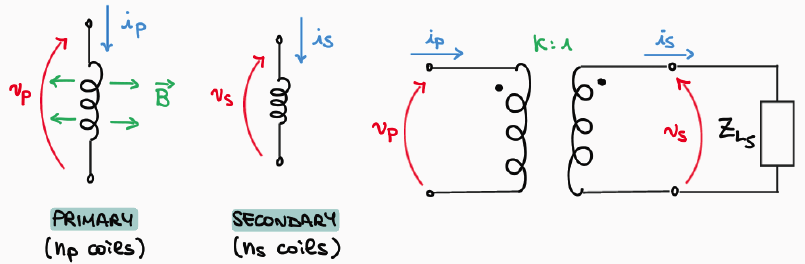
\includegraphics[width=0.65\linewidth]{signal_transformer.png}
    \caption{Ideal signal transformer with turns ratio \(k = n_p/n_s\). The voltage is scaled by \(k\) from primary to secondary; the current is scaled by \(1/k\). Power is conserved: \(v_p i_p = v_s i_s\)}
\end{figure}

\paragraph{Power grid example} A practical illustration of why the transformer is indispensable comes from electrical power transmission. Consider delivering \(P = \SI{1}{\mega\watt}\) of electrical power from a generating station to a city over a transmission line with resistance \(R_L\) per unit length. If the power is transmitted at low voltage (say \(v = \SI{10}{\kilo\volt}\)), the line current is \(i = P/v = \SI{100}{\ampere}\), and the resistive loss per kilometer is \(P_\mathrm{loss} = R_L i^2\), which at typical cable resistances amounts to roughly \SI{20}{\kilo\watt\per\kilo\meter}: a substantial fraction of the transmitted power. By inserting a step-up transformer at the generator to raise the voltage to \SI{380}{\kilo\volt}, the line current drops to \(i = P/v \approx \SI{2.6}{\ampere}\), and the resistive loss scales as \(i^2\), falling to approximately \SI{7}{\milli\watt\per\kilo\meter}: a reduction by a factor of nearly three million. A step-down transformer at the receiving end restores the voltage to a safe level for distribution. The transformer does not violate energy conservation; it simply trades current for voltage in a way that minimizes the dissipative penalty of line resistance.

\begin{figure}[!htb]
    \centering
    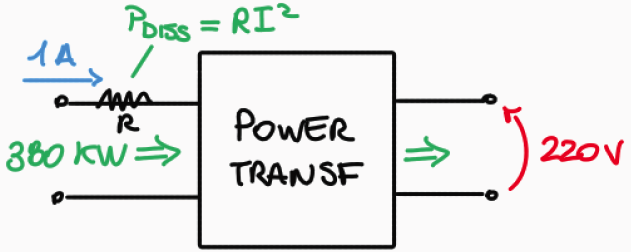
\includegraphics[width=0.8\textwidth]{power_transfer_block.png}
    \caption{High-voltage power transmission: a step-up transformer at the generator raises the voltage to \SI{380}{\kilo\volt} and reduces the current proportionally, cutting resistive line losses by the square of the voltage ratio. A step-down transformer restores usable voltage at the load}
\end{figure}

\subsection{Load Impedance Transformation}

A key property of the ideal transformer is that it modifies the impedance seen by the source. If the secondary port is loaded by an impedance \(Z_{LS} = v_s/i_s\), the impedance at the primary port is:
\[
Z_p = \frac{v_p}{i_p} = \frac{k v_s}{i_s/k} = k^2 \frac{v_s}{i_s}
\]
\begin{equation}
    Z_p = k^2 Z_{LS}
    \label{eq:impedanceTransform}
\end{equation}
A transformer with \(k > 1\) makes the load appear larger by a factor of \(k^2\) at the primary. This impedance scaling is exploited in audio engineering whenever the output impedance of a source must be matched to a load of different nominal impedance. A classic application is the output transformer of a vacuum-tube amplifier: the triode or pentode presents an output impedance of several kilohms, while a typical loudspeaker has a nominal impedance of \SI{4}{\ohm} to \SI{8}{\ohm}. The transformer scales the speaker impedance up so that it appears to the tube as the high-resistance load needed for efficient power transfer.
For example, a valve amplifier delivering \(P = \SI{100}{\watt}\) to a \SI{4}{\ohm} loudspeaker through a transformer with \(k = 20\) operates at primary voltage and current:
\[
i_p = \frac{i_s}{k} = \frac{5}{20} = \SI{250}{\milli\ampere}, \quad v_p = k v_s = 20 \times 20 = \SI{400}{\volt}
\]
The primary impedance is \(Z_p = k^2 Z_{LS} = 400 \times 4 = \SI{1600}{\ohm}\), a value compatible with the tube's operating point, while the secondary delivers the correct voltage and current to the speaker.

\begin{figure}[!htb]
    \centering
    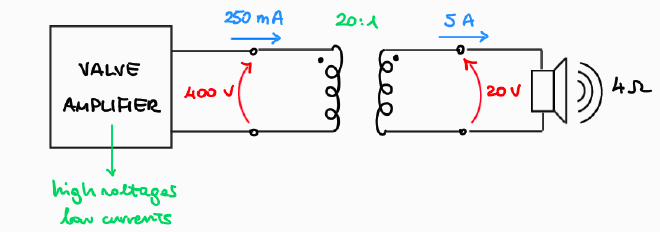
\includegraphics[width=0.6\linewidth]{valve_amp_to_loudspeaker.png}
    \caption{Impedance transformation in a valve amplifier: the output transformer scales the \SI{4}{\ohm} loudspeaker impedance up to \SI{1600}{\ohm} at the primary, matching the tube's operating conditions}
\end{figure}

\paragraph{Thevenin equivalent} When a Thevenin source with open-circuit voltage \(v_0\) and source impedance \(Z_0\) is connected to the primary, the equivalent Thevenin circuit seen from the secondary port has open-circuit voltage \(v_0/k\) and source impedance \(Z_0/k^2\). Both source voltage and source impedance are divided by \(k\) and \(k^2\) respectively when referred to the secondary side. This is a direct consequence of equation \eqref{eq:impedanceTransform} applied in reverse.

\begin{figure}[!htb]
    \centering
    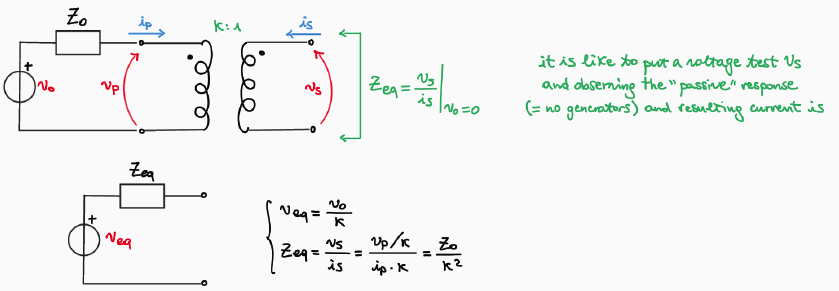
\includegraphics[width=0.75\linewidth]{Transformer_Thevenin_equiv.png}
    \caption{Thevenin equivalent of the signal transformer: a source \((v_0, Z_0)\) at the primary is seen from the secondary as a source \((v_0/k, Z_0/k^2)\)}
\end{figure}

\section{The Gyrator}
\label{sc:33}

The gyrator is a two-port network element introduced by Bernard Tellegen in 1948, the same researcher who formulated Tellegen's theorem in network theory and who is credited with conceiving the pentode vacuum tube. Tellegen proposed the gyrator as the fifth fundamental two-port, completing the canonical set of network elements alongside the resistor, capacitor, inductor, and transformer. Like the transformer, the gyrator is lossless: it transfers power from primary to secondary without dissipating energy. Unlike the transformer, it does not couple the two ports through a common magnetic flux but through a transconductance parameter \(g\) (in siemens, \(\si{\siemens} = \si{\ohm^{-1}}\)), which relates voltage on one port to current on the other in a crossed fashion.
The governing equations of the ideal gyrator are:
\begin{equation}
    i_s = g v_p, \qquad v_s = \frac{i_p}{g}
    \label{eq:gyratorLaws}
\end{equation}
from which it also follows that \(v_p = i_s/g\) and \(i_p = g v_s\). Power conservation is confirmed by:
\[
P_p = v_p i_p = \frac{i_s}{g}\cdot g v_s = v_s i_s = P_s
\]

\begin{figure}[!htb]
    \centering
    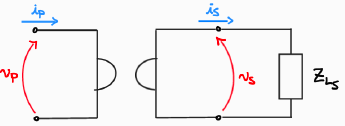
\includegraphics[width=0.45\linewidth]{gyrator_model.png}
    \caption{The ideal gyrator: transconductance \(g\) (in siemens) relates primary voltage to secondary current and vice versa. The element is lossless: \(v_p i_p = v_s i_s\)}
\end{figure}

\subsection{Impedance Inversion}
\label{ssc:331}

The most important property of the gyrator is impedance inversion. If the secondary port is loaded by an impedance \(Z_{LS} = v_s/i_s\), the primary input impedance is:
\[
Z_p = \frac{v_p}{i_p} = \frac{i_s/g}{g v_s} = \frac{1}{g^2}\cdot\frac{i_s}{v_s}
\]
\begin{equation}
    Z_p = \frac{1}{g^2 Z_{LS}} = \frac{Y_{LS}}{g^2}
    \label{eq:gyratorImpedance}
\end{equation}
The gyrator thus inverts the load impedance scaled by \(1/g^2\). This inversion exchanges the reactive nature of the secondary load as seen from the primary, with three notable consequences.

\paragraph{Resistive load} If \(Z_{LS} = R\), then \(Z_p = 1/(g^2 R) = G/g^2\) where \(G = 1/R\) is the load conductance. A resistor remains resistive at both ports, but its value is inverted.

\paragraph{Inductive load} If \(Z_{LS} = j\omega L\), then:
\[
Z_p = \frac{1}{g^2 j\omega L} = \frac{1}{j\omega C_\mathrm{eq}}, \qquad C_\mathrm{eq} = g^2 L
\]
An inductor at the secondary appears as a capacitor at the primary. This property is exploited in integrated-circuit design, where physical inductors are impractical: a gyrator loaded with a capacitor synthesizes a virtual inductor.

\paragraph{Capacitive load} If \(Z_{LS} = 1/(j\omega C)\), then:
\[
Z_p = \frac{j\omega C}{g^2} = j\omega L_\mathrm{eq}, \qquad L_\mathrm{eq} = \frac{C}{g^2}
\]
A capacitor at the secondary appears as an inductor at the primary. The gyrator therefore provides a complete duality between inductive and capacitive behavior.
The gyrator will reappear in Chapter 4 as the circuit representation of the electromechanical coupling in the impedance analogy: the motor law \(F = Bl i\) and the back-EMF law \(v = Bl u\) take precisely the form of equations \eqref{eq:gyratorLaws} with transconductance \(g = 1/(Bl)\).


\section{Domain Transductions}
\label{sc:41}

The loudspeaker pipeline connects three domains in sequence:
\[
\text{Electrical}\;(v, i)
\;\longrightarrow\;
\text{Mechanical}\;(F, u)
\;\longrightarrow\;
\text{Acoustical}\;(P, U)
\]
Each arrow represents a domain translation governed by the physical laws of the transduction mechanism. Both translations conserve instantaneous power in the lossless idealization.

\begin{figure}[!htb]
    \centering
    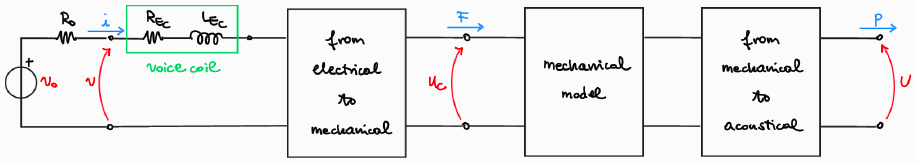
\includegraphics[width=0.90\textwidth]{loudspeaker_pipeline.png}
    \caption{The loudspeaker transduction chain: three physical domains linked by two domain translations. Each boundary is implemented as a two-port network element, either a transformer or a gyrator, depending on the analogy chosen}
\end{figure}

\subsection{Electrical to Mechanical Transduction}
\label{ssc:411}

The conversion from the electrical to the mechanical domain is governed by the Lorentz motor law. A current \(i\) flowing through a voice coil of effective length \(l\) in a magnetic field of flux density \(B\) generates the driving force:
\[
F_c = B l i
\]
Conversely, when the coil moves at velocity \(u_c\), a back-EMF is induced across the coil terminals according to Faraday's law:
\[
v = B l u_c \qquad \Longrightarrow \qquad u_c = \frac{v}{Bl}
\]
Written as a system, these two coupling equations are:
\[
\begin{cases}
    F_c = B l i \\[4pt]
    u_c = \dfrac{v}{B l}
\end{cases}
\]
Power is conserved across this translation: \(v i = (B l u_c) i = F_c u_c\), confirming that the electrical power input equals the mechanical power output in the lossless idealization.

\paragraph{Admittance analogy: transformer} Under the admittance analogy (\(F \leftrightarrow i\), \(u \leftrightarrow v\)), the coupling equations take the form:
\[
\frac{i}{F_c} = \frac{1}{Bl}, \qquad \frac{v}{u_c} = Bl
\]
This is exactly the transformer relation with turns ratio \(Bl\colon 1\). The primary port (electrical) carries current \(i\) and voltage \(v\); the secondary port (mechanical) carries force \(F_c \leftrightarrow i_s\) and velocity \(u_c \leftrightarrow v_s\).

\paragraph{Impedance analogy: gyrator} Under the impedance analogy (\(F \leftrightarrow v\), \(u \leftrightarrow i\)), the coupling equations become:
\[
i_s = g v_p \;\text{ with }\; g = \frac{1}{Bl}, \qquad v_s = \frac{i_p}{g}
\]
This matches the gyrator equations with transconductance \(g = 1/(Bl)\). The impedance analogy therefore represents the electromechanical coupling as a gyrator, and as a consequence of the impedance inversion property, the mechanical load impedance is inverted when referred to the primary electrical port.

\begin{figure}[!htb]
    \centering
    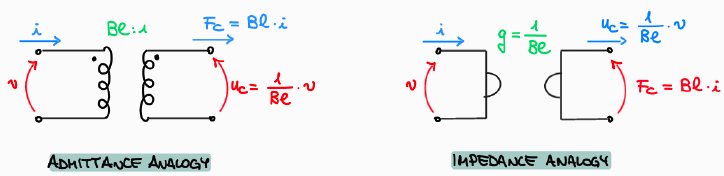
\includegraphics[width=0.70\linewidth]{imageE_M_analogies.png}
    \caption{Electrical-to-mechanical transduction under the admittance analogy (transformer with ratio \(Bl\colon 1\), left) and the impedance analogy (gyrator with \(g = 1/(Bl)\), right). The same physical law \(F = Bli\) is represented by two topologically different two-port elements}
\end{figure}

\subsection{Mechanical to Acoustical Transduction}
\label{ssc:412}

The conversion from the mechanical to the acoustical domain is governed by the geometry of the diaphragm. A diaphragm of area \(S_D\) translates mechanical force and velocity into acoustic pressure and volume velocity:
\[
\begin{cases}
    P = \dfrac{F}{S_D} \\[6pt]
    U = u S_D
\end{cases}
\]
Power is again conserved: \(P U = (F/S_D)(u S_D) = F u\). This translation has the form of a transformer with turns ratio \(1\colon S_D\) in both the admittance and impedance analogies.
%
%\begin{figure}[!htb]
%    \centering
%    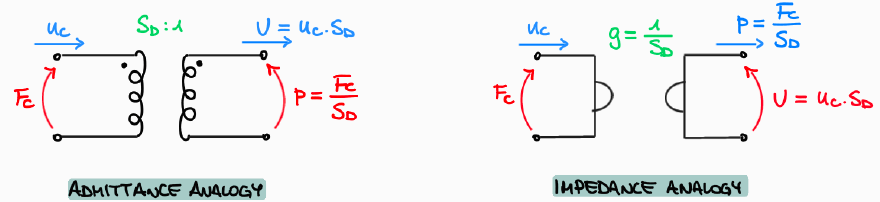
\includegraphics[width=0.80\linewidth]{M_A_Analogies.png}
%    \caption{Mechanical-to-acoustical transduction modeled as a transformer with ratio \(1\colon S_D\). The diaphragm area \(S_D\) sets the coupling in both analogies}
%\end{figure}

\section{Mechanical Section Modeling}
\label{sc:42}

The diaphragm and its suspension form the mechanical heart of the loudspeaker. The basket (frame) is mechanically rigid and is treated as the fixed reference, i.e., the ground node. The diaphragm of mass \(M_{MD}\) is connected to the basket through the suspension, which provides an elastic restoring force (modeled by the mechanical compliance \(C_{MS}\)) and viscous damping (modeled by the mechanical loss \(G_{MS}\)). The voice-coil velocity \(u_c\) equals the diaphragm velocity.
Three forces act on the diaphragm simultaneously: the spring restoring force \(F_S = x/C_{MS}\), where \(x = \int u dt\) is the displacement, giving \(u = C_{MS} dF_S/dt\); the damping force \(F_D = u / G_{MS}\); and the inertial force \(F_M = M_{MD} du/dt\). Applying d'Alembert's principle, the Lorentz driving force must balance the sum of all reaction forces at every instant:
\begin{equation}
    F_c = F_S + F_D + F_M = \frac{1}{C_{MS}}\int_0^t u(\tau) d\tau + R_{MS} u + M_{MD} \frac{du}{dt}
    \label{eq:dalembertDiaphragm}
\end{equation}

\paragraph{Admittance analogy: parallel RLC} Under the admittance analogy, velocity maps to voltage (\(u \leftrightarrow v\)) and force maps to current (\(F \leftrightarrow i\)). All three mechanical elements, the mass, the spring, and the damper, connect between the diaphragm node (at velocity \(u_c\)) and the basket node (at zero velocity). Because they all share the same velocity difference \(u_c\), they all have the same voltage in the equivalent circuit, which means they are connected in parallel. The driving force \(F_c\) is analogous to a current source, and by d'Alembert's equation \eqref{eq:dalembertDiaphragm} it is shared among the three parallel branches in direct analogy with Kirchhoff's current law at the diaphragm node. The mechanical section therefore maps to a parallel RLC circuit:
\[
M_{MD} \;\leftrightarrow\; C_{ED}, \qquad C_{MS} \;\leftrightarrow\; L_{ES}, \qquad G_{MS} \;\leftrightarrow\; R_{ES}
\]

\begin{figure}[!htb]
    \centering
    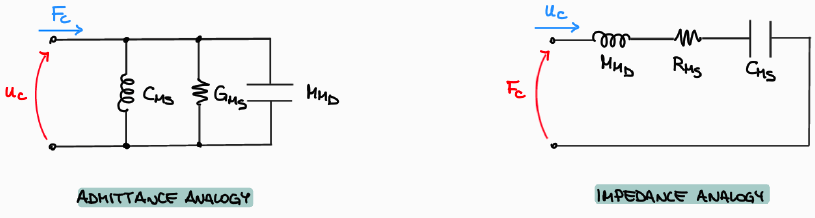
\includegraphics[width=0.85\textwidth]{mechanical_section_analogies.png}
    \caption{Mechanical section of the loudspeaker as a parallel RLC circuit (admittance analogy, left) and a series RLC circuit (impedance analogy, right). The admittance analogy is preferred because the parallel topology mirrors the actual physical arrangement: each element connects the moving diaphragm to the fixed basket}
\end{figure}

\paragraph{Impedance analogy: series RLC} Under the impedance analogy (\(F \leftrightarrow v\), \(u \leftrightarrow i\)), the common velocity \(u_c\) flows through all three elements in sequence, which is the analogue of Kirchhoff's voltage law for a series loop. The mechanical section maps to a series RLC circuit. The admittance analogy is nevertheless preferred for loudspeaker modeling, because the parallel topology visually preserves the physical arrangement of the mechanical system.

\section{The Full Equivalent Circuit and Impedance Reflection}
\label{sc:43}

Assembling all sub-models from the electrical input to the acoustic radiation port, the complete equivalent circuit of the loudspeaker in the admittance analogy consists of five cascaded stages:

\begin{enumerate}
    \item The voice coil is modeled as a series RL circuit with resistance \(R_{EC}\) (DC resistance of the winding) and inductance \(L_{EC}\) (inductance of the coil in the magnetic gap).
    \item The electrical-to-mechanical transduction is a transformer with turns ratio \(Bl\colon 1\).
    \item The mechanical section of the diaphragm-suspension assembly is a parallel RLC circuit.
    \item The mechanical-to-acoustical transduction is a transformer with turns ratio \(1\colon S_D\).
    \item The acoustic radiation environment is the radiation acoustic impedance \(Z_{AR} = \tilde{P}/\tilde{U}\).
\end{enumerate}

\begin{figure}[!htb]
    \centering
    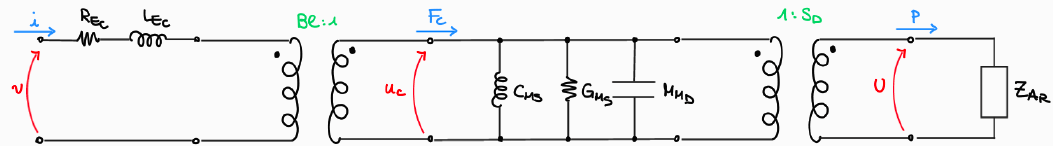
\includegraphics[width=0.95\textwidth]{loudspeaker_full_model.png}
    \caption{Complete equivalent circuit of the loudspeaker in the admittance analogy: voice-coil RL branch (\(R_{EC}\), \(L_{EC}\)), electromechanical transformer \(Bl\colon 1\), parallel RLC mechanical section (\(C_{MS}\), \(G_{MS}\), \(M_{MD}\)), mechano-acoustic transformer \(1\colon S_D\), and acoustic radiation admittance \(Y_{AR}\)}
    \label{fig:fullModel}
\end{figure}

\subsection{Referring All Elements to the Electrical Domain}
\label{ssc:431}

A practical strategy for circuit analysis is to reflect all elements through the transformers into a single domain, the electrical domain, eliminating both two-ports and obtaining a purely electrical network. The transformer relation \(v/i = (Bl)^2 u/F\) is used to convert each mechanical admittance to its electrical equivalent.

\paragraph{Diaphragm mass} Newton's second law gives \(F = M_{MD} du/dt\), so in the sinusoidal regime \(u/F = 1/(j\omega M_{MD})\). The electrical equivalent impedance is:
\[
\frac{v}{i} = (Bl)^2\cdot\frac{u}{F} = \frac{(Bl)^2}{j\omega M_{MD}} = \frac{1}{j\omega C_{ED}}, \qquad C_{ED} = \frac{M_{MD}}{(Bl)^2}
\]
The diaphragm mass corresponds to an equivalent electrical capacitance \(C_{ED}\). Since typical designs require \(C_{ED}\) of the order of nanofarads, a light diaphragm is desirable.

\begin{figure}[!htb]
    \centering
    \subfloat{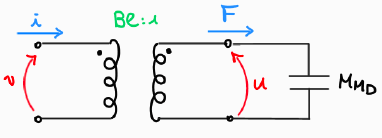
\includegraphics[height=0.15\textheight]{Diaphragm_capacitor_M_MD.png}}
    \hfill
    \subfloat{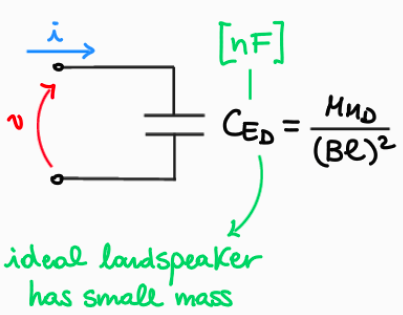
\includegraphics[height=0.15\textheight]{Diaphragm_capacitor_C_ED.png}}
    \caption{Diaphragm mass \(M_{MD}\) in the mechanical domain (left) and its electrical equivalent capacitance \(C_{ED} = M_{MD}/(Bl)^2\) (right). A lighter diaphragm produces a smaller \(C_{ED}\), which raises the resonance frequency}
\end{figure}

\paragraph{Suspension compliance} The compliance relation \(u = C_{MS} dF/dt\) gives \(u/F = j\omega C_{MS}\) in the sinusoidal regime. The electrical equivalent is:
\[
\frac{v}{i} = (Bl)^2\cdot j\omega C_{MS} = j\omega L_{ES}, \qquad L_{ES} = (Bl)^2 C_{MS}
\]
The suspension compliance corresponds to an equivalent electrical inductance \(L_{ES}\).

\begin{figure}[!htb]
    \centering
    \subfloat{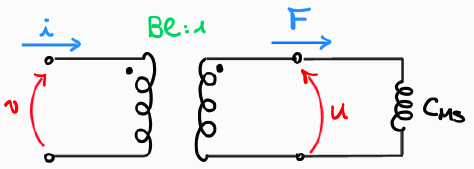
\includegraphics[height=0.12\textheight]{electrical_suspension_inductance.png}}
    \hfill
    \subfloat{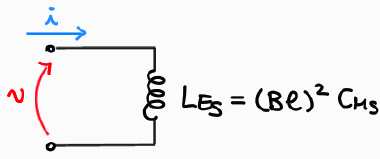
\includegraphics[height=0.12\textheight]{electrical_suspension_inductance_2.png}}
    \caption{Electrical equivalent of the suspension compliance: \(L_{ES} = (Bl)^2 C_{MS}\). A softer suspension (larger \(C_{MS}\)) produces a larger \(L_{ES}\) and lowers the resonance frequency}
\end{figure}

\paragraph{Suspension losses} The mechanical conductance \(G_{MS} = 1/R_{MS}\) gives \(u/F = G_{MS}\). The electrical equivalent is:
\[
\frac{v}{i} = (Bl)^2 G_{MS} \;\Longrightarrow\; R_{ES} = (Bl)^2G_{MS} = \frac{(Bl)^2}{R_{MS}}
\]
The suspension damping corresponds to an equivalent electrical resistance \(R_{ES}\). Note that a higher mechanical resistance (stronger damping) results in a lower \(R_{ES}\), because the bridge passes through a conductance.

\begin{figure}[!htb]
    \centering
    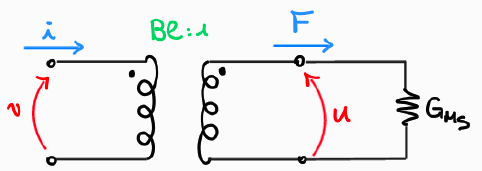
\includegraphics[width=0.70\linewidth]{electrical_suspension_resistance_0.png}
    \caption{Electrical equivalent of the suspension damping: \(R_{ES} = (Bl)^2/R_{MS}\). A more heavily damped suspension reduces \(R_{ES}\) and broadens the impedance resonance peak}
\end{figure}

\paragraph{Acoustic radiation impedance} The acoustic radiation admittance \(Y_{AR} = U/P\) is referred back to the electrical domain in two explicit steps.

\begin{enumerate}
    \item Acoustic to mechanical (transformer \(1\colon S_D\)): The mechano-acoustic coupling relations \(P = F/S_D\) and \(U = u\,S_D\) give directly:
    \[
    \frac{u}{F} = \frac{1}{S_D^2}\cdot\frac{U}{P}
    \qquad\Longrightarrow\qquad
    Y_{MR} = \frac{Y_{AR}}{S_D^2}
    \]
    Under the admittance analogy, \(Y_{MR} = u/F \leftrightarrow v/i = Z_{E}\), so the mechanical radiation admittance appears as an electrical impedance.
    \item Mechanical to electrical (transformer \(Bl\colon 1\)): The electromechanical coupling gives:
    \[
    \frac{v}{i} = (Bl)^2\cdot\frac{u}{F}
    \qquad\Longrightarrow\qquad
    Z_{ER} = (Bl)^2\,Y_{MR}
    \]
    Substituting the result of Step 1:
    \[
    Z_{ER} = (Bl)^2\cdot\frac{Y_{AR}}{S_D^2}
    = \left(\frac{Bl}{S_D}\right)^{2} Y_{AR}
    \]
\end{enumerate}

\subsection{The Overall Electrical Equivalent}
\label{ssc:432}

By combining all reflected elements, the complete loudspeaker reduces to a single electrical two-terminal network. The total electrical impedance decomposes as:
\[
Z_E = Z_{ES} + Z_{EM}
\]
where the series part collects the voice-coil elements:
\[
Z_{ES} = R_{EC} + j\omega L_{EC}
\]
and the parallel part groups the remaining reflected elements:
\[
Z_{EM} = Z_{L_{ES}}  ||  R_{ES}  ||  Z_{C_{ED}}  ||  Z_{ER}
\]

\begin{figure}[!htb]
    \centering
    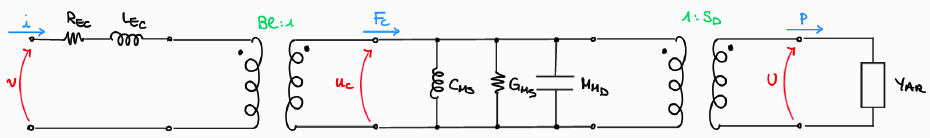
\includegraphics[width=0.90\textwidth]{overall_mechanical_model.png}
    \caption{Overall electrical equivalent circuit referred entirely to the electrical domain. Every mechanical and acoustical elements are represented by their electrical analogues}
\end{figure}

\begin{figure}[!htb]
    \centering
    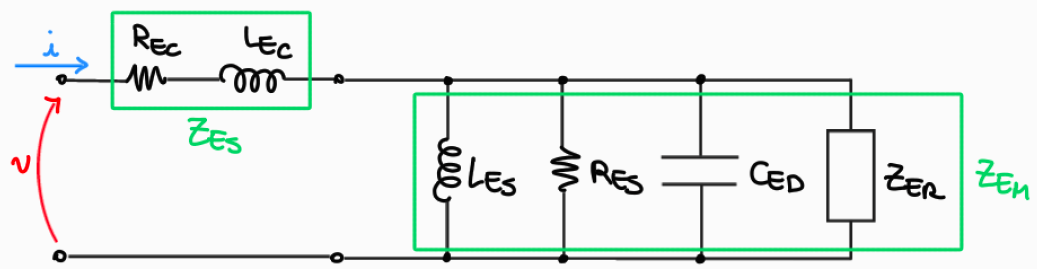
\includegraphics[width=0.70\textwidth]{overall_model_2.png}
    \caption{Simplified representation: the series block \(Z_{ES}\) and the parallel block \(Z_{EM}\) resonate at the fundamental frequency \(f_s\) of the diaphragm-suspension system}
\end{figure}

The parallel block \(Z_{EM}\) is a resonant RLC circuit. Its resonance frequency is:
\[
f_s = \frac{1}{2\pi\sqrt{L_{ES} C_{ED}}} = \frac{1}{2\pi\sqrt{(Bl)^2 C_{MS}\cdot M_{MD}/(Bl)^2}} = \frac{1}{2\pi\sqrt{M_{MD} C_{MS}}}
\]
which is precisely the fundamental mechanical resonance of the diaphragm-suspension system: the \(Bl\) factors cancel, confirming that \(f_s\) is a purely mechanical parameter independent of the magnetic circuit strength. At \(f = f_s\), the inductive and capacitive reactances in the parallel branch cancel and \(Z_{EM}\) reaches its maximum, which is the purely resistive value \(R_{ES}\). The total loudspeaker impedance therefore shows a pronounced peak at \(f_s\), the measurable feature used in practice to determine the Thiele-Small parameters of a driver.

\paragraph{Design implications of the model} The power of the equivalent-circuit approach lies in translating multi-physics design questions into familiar circuit terms. Doubling the diaphragm mass \(M_{MD}\) doubles \(C_{ED}\) and lowers \(f_s\) by \(\sqrt{2}\). Stiffening the suspension (reducing \(C_{MS}\)) reduces \(L_{ES}\) and raises \(f_s\). Weakening the magnetic gap (reducing \(Bl\)) lowers the transformer turns ratio, reducing coupling and increasing the effective mechanical load seen from the electrical terminals, thereby degrading efficiency. Increasing the diaphragm area \(S_D\) alters the acoustic transformer ratio and changes the reflected radiation impedance \(Z_{ER}\). All of these predictions follow from the circuit by inspection, without measurement or numerical simulation, which is the central advantage of the analogy-based modeling approach.
